\chapter{\IfLanguageName{dutch}{Fysieke proof-of-concept}{Fysieke proof-of-concept}}
\label{ch:Fysieke-proof-of-concept}

\section{Fysieke proof-of-concept}

Voor deze bachelorproef wordt een fysieke proof-of-concept opgesteld waarin meerdere hardwarecomponenten samenwerken om een testomgeving te realiseren. De opstelling is ontworpen om beide te scheiden en geen detectie mogelijk te maken aan de hand van locale software.

\section{Systeemopbouw}

De opstelling bestaat uit twee afzonderlijke computers:

\begin{itemize}
    \item \textbf{Game computer}: waarop de FPS-game wordt uitgevoerd.
    \item \textbf{Cheat computer}: waarop de verdere verwerking en analyse van het videobeeld plaatsvindt.
\end{itemize}

Door deze scheiding worden beide processen onafhankelijk van elkaar uitgevoerd, waardoor de detectie van de game computer geen cheats kan detecteren.

\section{Videodoorvoer}

Om het beeld van de game computer beschikbaar te maken op de cheat computer wordt gebruikgemaakt van een HDMI capture card. Deze hardwarecomponent ontvangt het HDMI-uitgangssignaal van de game computer en zet dit om naar een digitaal videosignaal dat via USB wordt doorgestuurd.
\\\\
Hierdoor wordt het beeld van de game computer real-time gespiegeld naar de cheat computer zonder softwarematige integratie tussen beide systemen.

\section{Inputsimulatie}

Voor het genereren van invoer wordt gebruikgemaakt van een Arduino Leonardo. Deze microcontroller ondersteunt native USB-emulatie, waardoor het apparaat door het besturingssysteem herkend wordt als standaard invoerapparaat.
\\\\
De Arduino wordt via USB verbonden met de game computer en functioneert als een emuleerbare muis. Hierdoor kan de microcontroller bewegingen en knopacties simuleren alsof deze afkomstig zijn van een fysiek randapparaat.
\begin{figure}[H]
    \centering
    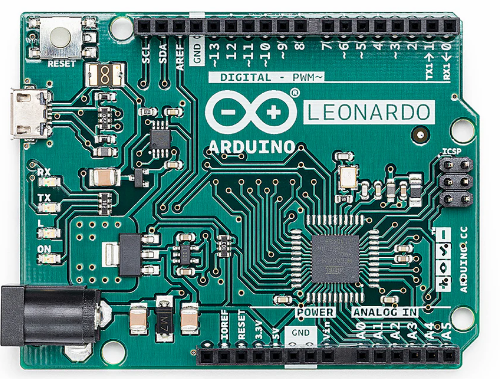
\includegraphics[width=0.6\textwidth]{../fotos/leonardo.png}
    \caption{Arduino Leonardo}
    \label{fig:leonardo}
\end{figure}

\section{Communicatie tussen systemen}

Om de communicatie mogelijk te maken tussen de cheat computer en de game computer aan de hand van de leonardo is er een andere arduino uno tussen de cheat computer en leonardo geplaatst.
De Arduino Leonardo bezit maar 1 poort waar de computer mee kan verbinden en is het niet mogelijk om ook rechtstreekt door te verbinden naar de game computer.
\\\\
Om dit op te lossen wordt er gebruik gemaakt van een Arduino Uno. Door de reset poort en de GND poort van de arudino uno te verbinden met elkaar wordt de chip uitgeschakelt en kan deze gebruikt worden als een USB-to-TTL converter.

Dit kan gebruikt worden om seriële communicatie mogelijk te maken tussen een computer en een microcontroller.

Zo kan de cheat computer toch communiceren met de Arduino Leonardo.
\begin{figure}[H]
    \centering
    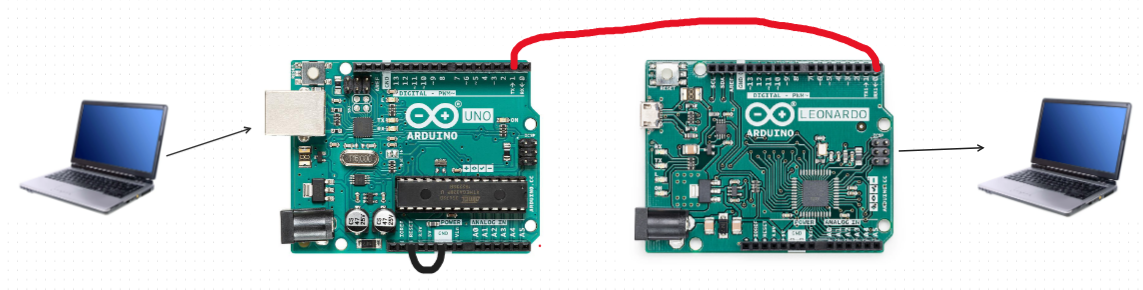
\includegraphics[width=1\textwidth]{../fotos/verbinding.png}
    \caption{verbinding tussen Arduino Uno en Arduino Leonardo}
    \label{fig:verbinding}
\end{figure}

\section{HID-emulatie}

De Arduino Leonardo wordt door het besturingssysteem herkend als een \textit{Human Interface Device} (HID). Hierdoor kan de microcontroller zich voordoen als een standaard invoerapparaat zoals een computermuis of toetsenbord.
\\\\
In tegenstelling tot klassieke Arduino-borden, zoals de Arduino Uno, beschikt de Leonardo over een ATmega32u4-microcontroller met ingebouwde USB-functionaliteit. Hierdoor kan het bord rechtstreeks communiceren met het besturingssysteem via het USB HID-protocol zonder bijkomende hardware.
\\\\
Wanneer de Arduino via USB verbonden wordt met de gamecomputer, detecteert het besturingssysteem het apparaat automatisch als een legitieme muis. Alle bewegingen die door de microcontroller gegenereerd worden, worden daardoor verwerkt als normale gebruikersinput op systeemniveau.
\\\\
Binnen deze proof-of-concept wordt de Arduino gebruikt om ontvangen seriële data om te zetten naar echte muisbewegingen. Hiervoor wordt gebruikgemaakt van de \texttt{Mouse.h}-library van Arduino, die HID-functionaliteit aanbiedt voor het simuleren van muisinvoer.
\\\\
De Arduino ontvangt via een seriële verbinding twee numerieke waarden die de horizontale en verticale muisverplaatsing voorstellen:

\[
(x, y)
\]

Deze waarden worden doorgestuurd vanaf een extern systeem en stellen de gewenste beweging van de muiscursor voor.
\\\\
Na ontvangst verwerkt de Arduino deze coördinaten en zet ze om naar HID-input via USB. Het besturingssysteem interpreteert deze bewegingen identiek aan fysieke input afkomstig van een echte computermuis.
\\\\
Omdat USB HID-rapporten beperkt zijn tot waarden tussen:

\[
-127 \leq x,y \leq 127
\]

worden grotere muisbewegingen automatisch opgesplitst in meerdere kleinere bewegingen. Hierdoor kunnen ook grote cursorverplaatsingen correct uitgevoerd worden zonder de HID-specificatie te overschrijden.
\\\\
Daarnaast bevat de implementatie een controlemechanisme dat valideert of volledige datapakketten correct ontvangen werden alvorens de beweging uit te voeren. Dit vermindert de kans op corrupte of onvolledige inputdata.
\\\\
De communicatie tussen beide systemen gebeurt via UART-seriële communicatie met een ingestelde baudrate van 9600 bits per seconde. Hierbij worden gegevens verzonden via de RX- en TX-pinnen van de Arduino Leonardo.
\\\\
Dankzij deze aanpak functioneert de Arduino als een hardwarematige brug tussen externe software en fysieke gebruikersinput. Hierdoor kunnen muisbewegingen gegenereerd worden zonder directe softwarematige interactie met het spelproces of het besturingssysteem.

\begin{minted}[fontsize=\small, linenos]{cpp}
#include <Mouse.h>

// Voor een Uno-bridge is 9600 de meest stabiele startwaarde
long BAUDRATE = 9600; 

void setup() {

  // USB-seriële communicatie voor debugging
  Serial.begin(BAUDRATE); 
  
  // Hardwarematige UART-communicatie
  Serial1.begin(BAUDRATE); 
  
  // Start HID-functionaliteit
  Mouse.begin();
}

void loop() {

  // Controleer of data beschikbaar is
  if (Serial1.available() > 0) {
    
    // Lees X- en Y-coördinaten
    int x = Serial1.parseInt();
    int y = Serial1.parseInt();
    
    // Controleer of datapakket correct eindigt
    if (Serial1.read() == '\n') {

      // Verdeel grote bewegingen in kleinere HID-pakketten
      while (x != 0 || y != 0) {

        int moveX = constrain(x, -127, 127);
        int moveY = constrain(y, -127, 127);

        // Verstuur HID-muisbeweging
        Mouse.move(moveX, moveY, 0);

        x -= moveX;
        y -= moveY;
      }
    }
  }
}
\end{minted}
\section{Samenvatting van de opstelling}

De volledige fysieke proof-of-concept bestaat uit:

\begin{itemize}
    \item een game computer voor het uitvoeren van de FPS-game;
    \item een HDMI capture card voor beelddoorvoer;
    \item een detectiecomputer voor verwerking van het videobeeld;
    \item een Arduino Leonardo voor USB HID-emulatie;
    \item een seriële communicatielink tussen detectiecomputer en microcontroller.
\end{itemize}

\begin{figure}[H]
    \centering
    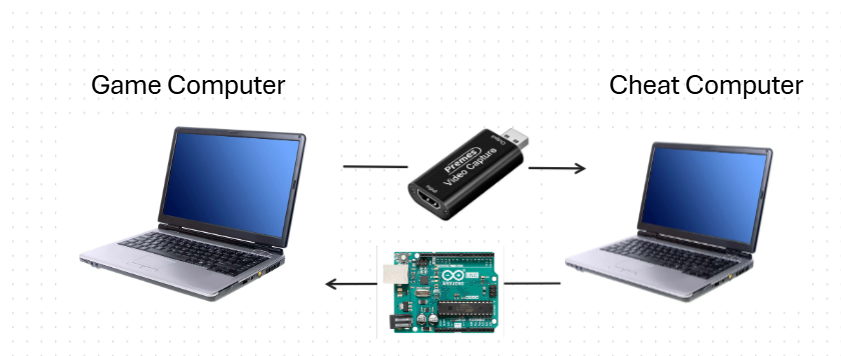
\includegraphics[width=0.6\textwidth]{../fotos/opstelling.png}
    \caption{Opstelling}
    \label{fig:Opstelling}
\end{figure}
Deze opstelling vormt een volledig gescheiden hardwarematige keten waarbij beeldinput en gebruikersinput via afzonderlijke componenten worden verwerkt.